\chapter{The LHCb Detector}
\label{chap:dec}

\textit{In this section, an overview of the accelerator complex at CERN as well as the physics motivation behind the \Gls{LHCb} detector and its design will be described.}

CERN has built one of the most exciting laboratories to study elementary particle interactions in the world. Its complex set of particle accelerators and detectors is shown in~\autoref{fig:AcceleratorComplex}. The process of accelerating protons starts with the source of protons. Protons are obtained from a hydrogen gas bottle by applying an electric field separating hydrogen into protons and electrons. The first proton accelerator in the chain, Linac 2, accelerates the protons to the energy of 50 \mev. Linac 2 is a tank composed of several chambers where the resonant cavities are tuned to a specific frequency creating potential differences in them, which then make the protons accelerate. The protons are then injected into the Proton Synchrotron Booster (\Gls{PSB}), where they are accelerated further to 1.4 \gev. The next in line is the Proton Synchrotron (\Gls{PS}) reaching \DIFaddbegin \DIFadd{an }\DIFaddend energy of 25 \gev. Before either entering the Large Hadron Collider (\Gls{LHC}) or North Area (mainly used as testing facility for experiment upgrades) the Super Proton Synchrotron (\Gls{SPS}) is the last accelerator in the chain. Here proton acceleration to 450 \gev is achieved.

\begin{figure}
  \centering
  \includegraphics[width=1.0\linewidth]{figs/detector/AccComplexpng2pdf_cropped.pdf}
	\caption{Accelerator complex at CERN. The image is taken from \cite{complex}.}
  \label{fig:AcceleratorComplex}
\end{figure}

\DIFaddbegin \DIFadd{The }\DIFaddend \Gls{LHC} is a complex machine which accelerates beams of protons in opposite directions in a $\sim$ 27km long circular tunnel. It is located
50-157\m below ground crossing the border between Switzerland and France. Once the desired energy is achieved proton-proton ($pp$) or ion collisions happen at four distinct points, where different detectors with different physics focus are located. These are \Gls{ATLAS}, \Gls{CMS}, \Gls{ALICE} and \Gls{LHCb}. 
The search for the decay \Bmumumu was performed using data obtained at \Gls{LHCb}\DIFaddbegin \DIFadd{\mbox{%DIFAUXCMD
\cite{det_paper}}%DIFAUXCMD
}\DIFaddend . 

\section{LHCb Layout }

\begin{figure}
	\centering
	\includegraphics[scale = 0.25]{figs/detector/lhcbdet.pdf}
	\caption{Schematic slice of \Gls{LHCb} detector in the $y,z$ plane where $z$ is defined to be the direction parallel to beamline, and $x,y$ define the plane perpendicular to the beamline. $\theta$, the opening polar in the y-z plane with $\theta$ = 0 along the $z-axis$. Figure from \cite{LHCbdetector}.}
	\label{fig:LHCbDetector}
\end{figure}


\Gls{LHCb}, seen in~\autoref{fig:LHCbDetector}, differs from the other general purpose detectors on the \Gls{LHC} ring as its main aim is to study properties of heavy particles containing $b$ or $c$ quarks. This is possible as this \DIFdelbegin \DIFdel{experiments }\DIFdelend \DIFaddbegin \DIFadd{experiment }\DIFaddend was designed to have \DIFdelbegin \DIFdel{the }\DIFdelend \DIFaddbegin \DIFadd{a }\DIFaddend geometrical acceptance and unique vertex resolution\DIFaddbegin \DIFadd{, }\DIFaddend as well as excellent particle identification (\Gls{PID})\DIFaddbegin \DIFadd{, }\DIFaddend suitable for beautiful and charming physics.

Studies of $B$ mesons can happen either at positron-electron colliders or at hadron colliders. The advantage of positron-electron \DIFdelbegin \DIFdel{collider }\DIFdelend \DIFaddbegin \DIFadd{colliders }\DIFaddend is that the information about all the event is known, as just two $B$ mesons and nothing else is produced in \DIFaddbegin \DIFadd{the }\DIFaddend collisions. This gives an overall constraint on collision information, unlike in the hadron collider $B$ factory, \gls{LHCb}. Contrary to the two general purpose detectors at \gls{LHC}, where the collisions \DIFdelbegin \DIFdel{are occurring }\DIFdelend \DIFaddbegin \DIFadd{occur }\DIFaddend in the centre of the detector, \Gls{LHCb}'s collision point is located at one end of the detector, hence its description as a forward single-arm spectrometer. 

The disadvantage of not having an overall constraint on collision information is, however, compensated by the production mechanism of $b\bar{b}$ and $c\bar{c}$ in $pp$ interactions, which occurs predominantly via gluon-gluon fusion. In this process, each gluon will carry part of proton's momentum. If the two gluons from two protons carry significantly different \DIFdelbegin \DIFdel{momentum}\DIFdelend \DIFaddbegin \DIFadd{momenta}\DIFaddend , the $b\bar{b}$ system will be boosted with respect to the $pp$ rest frame, either in the forward or backward cone \DIFdelbegin \DIFdel{closely }\DIFdelend \DIFaddbegin \DIFadd{close }\DIFaddend to the beamline, as can be seen in~\autoref{fig:Acceptance}(b).


\begin{figure}
	\centering
	\includegraphics[width=0.45\linewidth]{figs/detector/license/croped.pdf}%
	\includegraphics[width=0.5\linewidth]{figs/detector/Acceptance.pdf}\put(-10,170){(b)}
	\caption{(a) Probability of interaction per bunch crossing as a function of instantaneous luminosity. Figure from \cite{Raven:2007zi}. (b) Angular production and acceptance of the $b$ (x-axis) $\bar{b}$ (y-axis) pair produced from \DIFaddbeginFL \DIFaddFL{a }\DIFaddendFL $pp$ collision at the LHC. The acceptance of the LHCb detector is the red box and the acceptance of the General Purpose Detector is shown in the yellow box. \Gls{LHCb} covers the region with highest production cross-section at 8 \tev. These plots were produced using a Pythia 8.1 \cite{pythia8} simulation. Figure from \cite{acceptance}.}
	\label{fig:Acceptance}
\end{figure}

The angular coverage of \Gls{LHCb} is formally defined using pseudorapidity $\eta$, 

\begin{equation}
	\eta = -\ln \Big(\tan\frac{\theta}{2}\Big)
\end{equation}	
where $\theta$ is the polar angle measured from the beam axis. The \Gls{LHCb} detector was built to cover the region $2<\eta<5$. The production cross-section of the fundamental process of $pp\rightarrow b\bar{b}X$ was measured in this region yielding, $\sigma (pp\rightarrow b\bar{b}X)$= 75.3$\pm$5.4$\pm$13.0 $\mub$ at 7 \tev \cite{LHCb-PAPER-2010-002} and 144$\pm$1$\pm$21 $\mub$ at 13 \tev \cite{LHCb-PAPER-2016-031}, which shows that the production cross-sections scales roughly linearly with the centre-of-mass energy. Assuming \DIFaddbegin \DIFadd{the }\DIFaddend design conditions of \gls{LHCb}, listed in~\autoref{tab:runcond}, 2$\fb^{-1}$ of data (eqvivalent to \DIFaddbegin \DIFadd{the }\DIFaddend 2012 dataset) would correspond to $10^{12}$ \DIFdelbegin \DIFdel{of }\DIFdelend $b\bar{b}$ pairs being produced in a full 4$\pi$ region with 27\% of these $b\bar{b}$ pairs produced in the \gls{LHCb} acceptance. The summary of \gls{LHCb} running conditions is also provided in~\autoref{tab:runcond}. The analysis of \Bmumumu is done with \DIFaddbegin \DIFadd{the }\DIFaddend Run \Rn{1} and 2016 dataset. 

Despite the impressive statistics of $b\bar{b}$ pairs available to \Gls{LHCb}, the bottleneck in terms of data collection arises from the much more copious inelastic background. That mostly originates from soft \gls{QCD} processes which are related to the amount of pile-up, the visible number of $pp$ \DIFdelbegin \DIFdel{interaction }\DIFdelend \DIFaddbegin \DIFadd{interactions }\DIFaddend in the visible events. By looking at the probability of the number of $pp$ interaction per bunch crossing as a function of luminosity, shown in~\autoref{fig:Acceptance}(a), it can be noted that the maximum probability for only one $pp$ interaction (and hence minimizing the background) is found to be at $\sim 2 \times10^{32} \mathrm{cm^{-2} s^{-1}}$.  This was the reason behind \DIFaddbegin \DIFadd{the }\DIFaddend \gls{LHCb} design luminosity. Subsequently it has been found that it is more optimal to run at a higher luminosity of $\sim 4 \times10^{32} \mathrm{cm^{-2} s^{-1}}$ but then implement a set of global event cuts (GEC). Only events with 600 (in 7,8 \tev) and 450 (in 13 \tev) hits and less, corresponding to the track density in the particular part of the detector, are allowed to be processed.
As the majority of the branching fractions at \gls{LHCb} are measured with respect to other branching fractions, there is no bias \DIFdelbegin \DIFdel{being }\DIFdelend introduced by the GECs. 

As \Gls{LHCb} requires much lower luminosity compared to other \gls{LHC} detectors, there is an LHCb-specific control of luminosity known as \textit{luminosity levelling}, shown in~\autoref{fig:lhcbintlumi}. This procedure achieves stable instantaneous luminosity by controlling that the two beams do not collide straight head-on at collision point, but are moved with respect to each other. It limits the effects of luminosity decay, which can lead to trigger alterations during specific data taking run, resulting in systematic uncertainties.



%The summary of \gls{LHCb} running conditions is provided in~\autoref{tab:runcond}, showing the evolution of the instantaneous luminosity as well as the frequency of collisions compared to the design proposal.
%Formally \Gls{LHCb}   detector is placed along the beamline, where $x,y,z$ a spectrometer which cover the region of 300 \mrad defined a
%http://lhcb.web.cern.ch/lhcb/speakersbureau/excel/default.html

%\begin{figure}
%	\centering
%	\includegraphics[scale = 0.5]{figs/detector/lumicompare.png}
%	\caption{Integrated luminosity collected in different years of data-taking. This plot is taken from \cite{lumiover}.}
%	\label{fig:lhcbintlumi}
%\end{figure}



\begin{table}[!h]
	\centering
%	\hspace*{-0.8cm}
	\begin{tabular}{l c c c }
		\toprule
		Year & $\sqrt{s}$ & $\mathcal{L}$  & Integrated Recorded Luminosity \\ 
		 & [\tev] & [$\times10^{32} \rm{cm^{-2}s^{-1}}$] & [$\rm{fb}^{-1}$] \\ \hline
		Design & Up to 14 & 2 & - \\
		2011  \rdelim\}{2}{1.5cm}[Run \Rn{1}] & 7 & $\sim$ 3.0-3.5 & 1.1 \\
		2012 & 8 & $\sim$ 4.0 & 2.1 \\
		2015 \rdelim\}{3}{1.5cm}[Run \Rn{2}] & 13 & $\sim$ 0.5-4.5 & 0.3 \\      
		2016 & 13 & $\sim$ 4.0 & 1.7  \\      
		2017 & 13 & $\sim$4.0-6.0 & 1.7 \\\bottomrule      
	\end{tabular}
	\caption{Running conditions of \gls{LHC} and \Gls{LHCb} in different years of data-taking. The statistics of \gls{LHCb}'s instantaneous luminosity, $\mathcal{L}$ is extracted using run database information. Run \Rn{2} data-taking finishes in 2018.}
	\label{tab:runcond}
\end{table}   

\begin{figure}
	\centering
%	\includegraphics[width = 0.5\textwidth]{figs/detector/intlumi.png}\put(-15,100){(a)}
        \includegraphics[width = 0.65\textwidth]{figs/detector/lumicompare.png}%\put(-15,100){(b)}
	%\caption{(a) Integrated luminosity collected in different years of data-taking. This plot is taken from \cite{lumiover}. (b)
	\caption{Development of the instantaneous luminosity for \Gls{ATLAS}, \Gls{CMS} and \Gls{LHCb} during \DIFaddbeginFL \DIFaddFL{random representative }\DIFaddendFL LHC fill\DIFdelbeginFL \DIFdelFL{2651. }\DIFdelendFL \DIFaddbeginFL \DIFaddFL{. }\DIFaddendFL After ramping to the desired value of $4\times10^{32}\mathrm{cm^{-2}s^{-1}}$
	for \Gls{LHCb}, the luminosity is kept stable in a range of 5$\%$ for about 15 hours by adjusting the transversal beam overlap. The difference in luminosity towards the end of the fill between \Gls{ATLAS}, \Gls{CMS} and \Gls{LHCb} is due to the difference in the final focusing at the collision points, commonly referred to as the beta function, $\beta^{*}$. This plot was obtained from \cite{LHCb-DP-2014-002}.}
	\label{fig:lhcbintlumi}
\end{figure}

In the following sections, a brief discussion of the different subdetectors, shown in~\autoref{fig:LHCbDetector}, is presented. The vertexing at \gls{LHCb} is performed with the vertex locator system, also known as the VELO, \DIFaddbegin \DIFadd{and }\DIFaddend is described in~\autoref{velosys}. The tracking system at \gls{LHCb} consisting of trackers before \DIFaddbegin \DIFadd{the }\DIFaddend magnet (TT), and three tracking stations behind the magnet (T1, T2, T3) is highlighted in~\autoref{tracksys}. The particle identification is provided by two Ring Imaging \v{C}erenkov counters (RICH1 and RICH2), which are detailed in~\autoref{richsec}. No particle physics experiment is complete without a calorimeter system, discussed in~\autoref{calosys}, which consists of a Scintillator Pad Detector (SPD), Preshower (PS), an electromagnetic calorimeter (ECAL) and finally a hadronic calorimeter (HCAL). The muon system positioned at the end of the detector, consisting of five muon chambers is described in~\autoref{muonsys}. The trigger chain as well as the simulation chain are discussed in~\autoref{triggerchap} and~\autoref{simulationchap}. Particular emphasis is given to the muon detectors and the simulation of \gls{LHCb}.

%\color{red}{ \mybox{Sally} corrected until now} \color{black}.

\section{VErtex LOcator }
\label{velosys}
The subdetector closest to the collision point is the VErtex LOcator (\Gls{VELO}). This silicon-strip based detector, that extends 1 \m along the beam axis, is primarily used to distinguish signal-like events from prompt background. The typical \DIFdelbegin \DIFdel{differing }\DIFdelend property of a $b$-hadron decay \DIFdelbegin \DIFdel{includes }\DIFdelend \DIFaddbegin \DIFadd{include }\DIFaddend large impact parameter (\Gls{IP}), the minimal distance between the track and a primary vertex, in addition to significantly higher transverse momentum, $p_{T}$. Therefore, the main tasks of this subdetector \DIFdelbegin \DIFdel{is }\DIFdelend \DIFaddbegin \DIFadd{are }\DIFaddend to find: 
 \begin{itemize} 
\item primary vertices
\DIFdelbegin \DIFdel{positions
}\DIFdelend \item secondary vertices of short-lived particles (heavy quark hadrons)
\item tracks that did NOT originate from \DIFaddbegin \DIFadd{the }\DIFaddend primary vertex
 \end{itemize} .


\begin{figure}[!h]
	\centering
	\includegraphics[width = 0.75\textwidth]{figs/detector/license/Velo_croped.pdf}
        %\includegraphics[width = 0.5\textwidth]{figs/detector/lumicompare.png}
	\caption{Schematic plot of the \Gls{VELO} detector configuration along the beam pipe showing the layout as well as positions while in stable beams (discs have slight overlap) and injection. Figure from \cite{det_paper}.}
	\label{fig:veloover}
\end{figure}

The detector consists of two sets of 21 silicon modules positioned around the beam pipe, where each module has 2 types of half-moon-shaped discs as seen in~\autoref{fig:veloover}. In the first type, the strips are arranged to provide radial information ($R$), whereas the second type provides azimuthal ($\phi$) information. As $pp$ collisions bring a high dose of radiation to this detector, the first sensitive strip starts at a distance of 8 \mm once stable beams are declared. Throughout the beam injection, when the beam radius may be larger, the two sets are moved 3 \cm away, perpendicular to the beam axis. For the $R$ sensor, the individual module's strip pitch, the distance between two strips, varies from 38 $\mum$ to 102 $\mum$ away from the beam pipe, so that the hit occupancy is roughly even as a function of distance away from the beam pipe. Each \Gls{VELO} half is kept within an aluminium welded box causing material overlap once stable beams are declared. These boxes form their own vacuum which is separated from the nominal \gls{LHC} vacuum in order to protect the detector from any electromagnetic interference with the beam. 

This setup brings outstanding hit resolution (4-40$\mum$), which in turn allows for very high \gls{IP} and very good primary vertex (\gls{PV}) resolution, as seen in~\autoref{fig:veloIPres}(a)(b). This is indispensable not only in order to perform the precise measurements of $B$ and $D$ lifetimes, but also to resolve oscillations caused by $B^{0}_{s}-\bar{B}^{0}_{s}$ mixing occurring at a 3 trillion \hz rate. As will be seen later, this excellent resolution is also very important for the detection of decays with neutrinos in the final state.

\begin{figure}[!h]
	\centering
	\includegraphics[width = 0.5\textwidth]{figs/detector/IPRes-Vs-P-CompareIPxIPy-2012.pdf}\put(-50,70){(a)}
        \includegraphics[width = 0.5\textwidth]{figs/detector/ResXY_1PV_2011Data.pdf}\put(-50,70){(b)}
	\caption{Two key variables which quantify performance of the \Gls{VELO} detector. (a) \Gls{IP} resolution which is worse for low momentum tracks and (b) \Gls{PV} resolution dependent on the number of tracks forming the primary vertex $N$. Figures from \cite{LHCbVELOGroup:2014uea}.}
	\label{fig:veloIPres}
\end{figure}


\section{Tracking System }
\label{tracksys}
In addition to tracking information provided by the \Gls{VELO}, the trajectories of charged particles are measured by a series of tracking subdetectors. The main task of these tracking subdetectors is to provide efficient reconstruction and precise measurement of a particle's momentum. There are four tracking stations apart from \Gls{VELO}: Tracker Turicensis (\Gls{TT}), positioned upstream from the magnet, and the \Gls{Tstation} tracking stations on the other side of the magnet. The dipole magnet with $\approx$ 4 Tm integrated field provides strength to bend charged particles in \DIFaddbegin \DIFadd{the }\DIFaddend horizontal plane.
% 10 m of charged trakcs
%with $p$ of 200 $\gev/c^{2}$.      

 Two different detection technologies are used in these trackers reflecting the nature of track occupancy as a function of polar angle. The \DIFdelbegin \DIFdel{tracker's part }\DIFdelend \DIFaddbegin \DIFadd{parts }\DIFaddend at small polar angles, \Gls{TT} station together with central region of \Gls{Tstation}, also known as \DIFaddbegin \DIFadd{the }\DIFaddend Inner Tracker (\Gls{IT}), \DIFdelbegin \DIFdel{expects }\DIFdelend \DIFaddbegin \DIFadd{expect }\DIFaddend higher occupancy and \DIFdelbegin \DIFdel{makes }\DIFdelend \DIFaddbegin \DIFadd{make }\DIFaddend use of the silicon microstrip detection mechanism. The outer part of \Gls{Tstation} stations, also known as the Outer Tracker (\Gls{OT}), is made of straw-tube detectors. Straw tubes measure the trajectory of the track by measuring the drift-time of ionized electrons. Use of the two technologies is illustrated in~\autoref{fig:tracktype}(a). 

\subsection{Tracking Algorithms} 
Different types of particles will leave different footprints in the detector. Charged particles will form tracks. Depending on the presence of hits in individual subdetectors, they are grouped into several categories, visualized in~\autoref{fig:tracktype}(b).

\begin{figure}[!h]
	\centering
	\includegraphics[width = 0.35\textwidth]{figs/detector/license/OT_crop.pdf}\put(-30,90){(a)}%
	\includegraphics[width = 0.6\textwidth]{figs/detector/tracktype.png}\put(-30,90){(b)}
	\caption{ (a) Visualisation of use of different technology with silicon technology in violet and straw-tube technology in cyan. Figure from \cite{det_paper}. (b) Track types categorisation depending on which track stations provided hits. For the study of \Bmumumu decays, only \gls{longtrack}s are considered as muons will travel to the end of the detector leaving \DIFdelbeginFL \DIFdelFL{the }\DIFdelendFL hits all along. Figure from \cite{LHCb-DP-2013-002}.}
	\label{fig:tracktype}
\end{figure}

%http://iopscience.iop.org/article/10.1088/1748-0221/3/08/S08005/pdf
%https://twiki.cern.ch/twiki/bin/view/LHCb/TrackingEffAbsLength /secondary interactions - hadronic int.

Most of the physics analyses at \gls{LHCb}, as it is the case for the search of \Bmumumu, use only \gls{longtrack}s, tracks leaving hits in the \Gls{VELO} and \Gls{Tstation}, as they give most precise momenta measurements. There are also other types of tracks as indicated in~\autoref{fig:tracktype} but they are rarely used.
%VELO tracks leave hits only in $R$ and $\Phi$ sensor, but not in any other tracking stations. VELO tracks are formed by particles which must have left \Gls{LHCb} acceptance or they come from particles produced backwards and hence are useful for \gls{PV} reconstruction. Upstream tracks are formed by tracks leaving hits in \Gls{VELO} and \gls{TT} only. These are usually low momentum particles, which are bent out \Gls{LHCb} acceptance while traversing the magnet. Long-lived particles such as $\Lambda$ or $K^{0}_{s}$ will only decay outside of the \Gls{VELO} acceptance and hence will produce no hits until \Gls{TT} and \Gls{Tstation} forming downstream tracks. T-track is track type that only have hits in \Gls{Tstation}. Again this could be due to presence of long-lived particles or due to secondary interactions in the detector.   

In general, the track reconstruction software starts with \textit{pattern recognition}, where several hits in one part of a tracking subdetector are identified and form \textit{track seeds}, which are then extrapolated and combined with hits in other tracking subdetectors. The long track candidates are formed and fitted with a Kalman filter\cite{Hierk:684697}, where, because of the material present in the detector, corrections for energy losses as well as multiple scattering are incorporated.

In \gls{LHCb} there are types of tracks which are not really the trajectories of charged particles.
Sometimes the \textit{pattern recognition} may combine random hits into a track, which is then known as a \textit{ghost track}. On the other hand, it could also happen that several tracks are sharing the same hits, known as \textit{clone tracks}. The presence of these types of tracks are suppressed through the use of a neural network based variable (\Gls{pgh2}), which relies on \DIFaddbegin \DIFadd{the }\DIFaddend $\chi^{2}$ of the track fit, and information about missing hits along the trajectory to calculate its value.
%Presence of these tracks are heavily suppressed with different techniques - such as establishing ghost probability (\Gls{pgh2})- variable based on the output of neural network combining track $\chi^{2}$, quality of the track, and missing hits in the subdetectors.

When searching for a $b$-hadron decay, the mass of a candidate can be calculated from the 4-momenta of the decay products. Uncertainty on this mass is one of the crucial parameters to minimize as it enables a better separation between the identified signal and background. It strongly correlates with \DIFaddbegin \DIFadd{the }\DIFaddend momentum resolution that is obtained using \DIFaddbegin \DIFadd{the }\DIFaddend tracking system. \DIFdelbegin \DIFdel{Resulting }\DIFdelend \DIFaddbegin \DIFadd{The resulting }\DIFaddend relative momentum uncertainty (0.5-1.1\%) on \gls{longtrack}s using $J/\psi \rightarrow \mu^{+} \mu^{-}$ data can be seen in~\autoref{fig:momres}. It varies logarithmically with increasing momentum.


\begin{figure}[!h]
	\centering
	\includegraphics[width = 0.6\textwidth]{figs/detector/Fig17.pdf}
	\caption{Momentum resolution of \gls{longtrack}s measured at \gls{LHCb}. The decay channel $J/\psi \rightarrow \mu^{+} \mu^{-}$ is analysed for this purpose. Figure from \cite{LHCb-DP-2014-002}.}
	\label{fig:momres}
\end{figure}

\section{Ring Imaging \v{C}erenkov Detectors}
\label{richsec}
Particle identification, \Gls{PID}, at \Gls{LHCb} relies heavily on two dedicated Ring Imaging \v{C}erenkov subdetectors, \gls{RICH}. These detectors take advantage of the emission of \v{C}erenkov light, which happens when a charged particle travels through a medium at a speed faster than the phase velocity of light in that medium. This cone of light is emitted at an angle $\theta$ with respect to the charged particle's trajectory. Using the knowledge of \DIFaddbegin \DIFadd{the }\DIFaddend refractive index of the medium, $n$, and momentum $p$ that is measured using the tracking system, the mass $m$ of the particle can be obtained through:

\begin{equation}
	\cos\theta_{c} =  \frac{\sqrt{m^{2} + p^{2}}}{pn}.
\end{equation}

As the momentum is not an intrinsic property of a passing particle, the momentum identification range is limited by the choice of medium, also known as radiator. For very low-momentum particle, as $\cos\theta_{c} \rightarrow 1$ ($p=\sqrt{\frac{m^{2}}{n^{2}-1}}$), the particle is not producing any \v{C}erenkov light cone. At \DIFdelbegin \DIFdel{the }\DIFdelend very high momentum, as $\cos\theta_{c} \rightarrow 1/n$, there is \DIFaddbegin \DIFadd{a }\DIFaddend saturation point as all species of \DIFdelbegin \DIFdel{particles will emit the }\DIFdelend \DIFaddbegin \DIFadd{particle will emit }\DIFaddend light at the same \v{C}erenkov angle, hence all the discriminating power will be lost.

Low momentum (2-60 \gev) particles are identified in the upstream \gls{RICH1} detector and high momentum particles (15-100) \gev are analyzed downstream in \gls{RICH2}. \gls{RICH1} covers \DIFaddbegin \DIFadd{an }\DIFaddend angular acceptance of 25-300 mrad using $\rm{C_{4}F_{10}}$ ($n = 1.0014$) as \DIFaddbegin \DIFadd{the }\DIFaddend radiator. \gls{RICH2} has \DIFaddbegin \DIFadd{a }\DIFaddend more limited acceptance of 15-120 mrad and uses $\rm{CF_{4}}$ as \DIFaddbegin \DIFadd{the }\DIFaddend radiator, with lower $n=1.0005$. The discrimination power between different particles can be seen in~\autoref{fig:richres}(a). 


Both \gls{RICH1} and \gls{RICH2} use a set of spherical primary mirrors to guide the photons onto the flat secondary mirrors which are then further focused into \v{C}erenkov rings on the surface of a plane of Hybrid Photon Multipliers, (\Gls{HPD}). The schematic view of a particle passing through \gls{RICH1} can be seen in~\autoref{fig:richres}(b). 


\begin{figure}[!h]
	\centering
	\includegraphics[width = 0.5\textwidth]{figs/detector/CKAnglevsMom_NoTheory_jun2011-01.eps}\put(-50,170){(a)}%
	%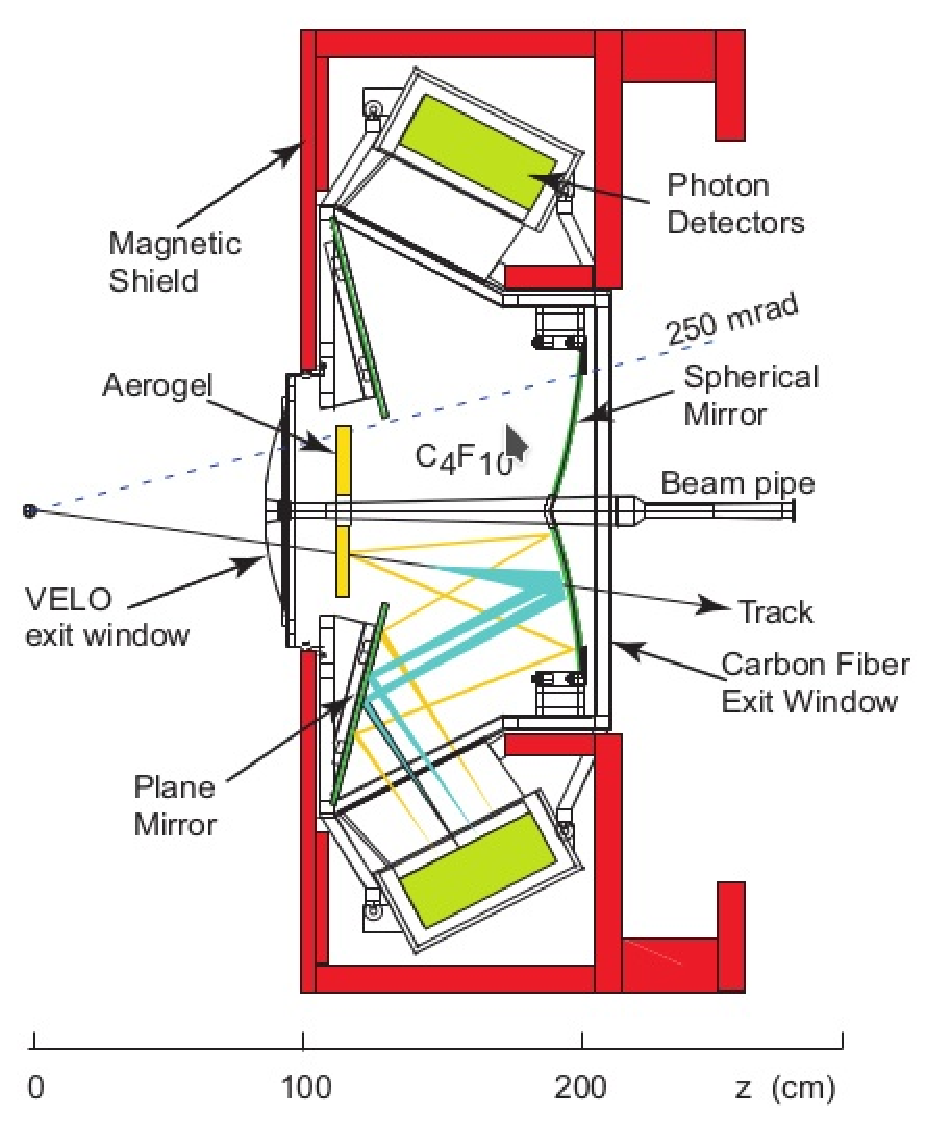
\includegraphics[width = 0.4\textwidth]{figs/detector/mechrich.eps}%
	\includegraphics[width = 0.4\textwidth]{figs/detector/license/Rich_croped.pdf}\put(-10,170){(b)}%
	\caption{ (a) Separation power for different species of particles in \DIFaddbeginFL \DIFaddFL{the }\DIFaddendFL momentum-\v{C}erenkov angle plane for \DIFaddbeginFL \DIFaddFL{the }\DIFaddendFL $\rm{C_{4}F_{10}}$ radiator. Figure from \cite{LHCb-DP-2012-003}. (b) Schematic diagram of \gls{RICH1} layout. Figure from \cite{det_paper}.}
	\label{fig:richres}
\end{figure}

\section{RICH Reconstruction and Performance }
In order to \DIFdelbegin \DIFdel{establish }\DIFdelend \DIFaddbegin \DIFadd{correctly associate }\DIFaddend species of particles \DIFdelbegin \DIFdel{for each }\DIFdelend \DIFaddbegin \DIFadd{to a given }\DIFaddend track, the \v{C}erenkov angle is combined with the track momentum measured by tracking. In practice, however, as \Gls{RICH} detectors operate in high track density environment, many \v{C}erenkov rings will be overlapping and hence a complex pattern recognition algorithm is deployed \cite{Forty:1999sg}. 


For each event, the \Gls{RICH} computes a full event likelihood that is consistent with assigning a pion mass hypothesis to all tracks given the observed hit distribution read out by the \Gls{HPD}s. The algorithm then iterates through all other possible particle species, ($e, \mu, \pi, K,$ proton, deuteron), assigning a new full event likelihood for a given track, \DIFdelbegin \DIFdel{having }\DIFdelend \DIFaddbegin \DIFadd{with }\DIFaddend all other hypotheses fixed. The mass hypothesis with the highest full event likelihood is assigned to the track and this process is repeated for all the tracks in the event, until no improvement is found. 

Results of this algorithm provide likelihood variables, $\rm{\textrm{DLL{x}}}$, that quantify the strength of the chosen species hypothesis against the pion hypothesis,
\begin{equation}
	\textrm{\textrm{DLL{x}}} = \mathrm{log}(\mathcal{L})_{x} - \mathrm{log}(\mathcal{L})_{\pi} \quad  x\in{e, \mu, K, \rm{proton, deuteron}}.
\end{equation}

By calculating $\rm{DLL{x_{1}} - DLL{x_{2}}}$, one can obtain discriminative strength between any two species.

\subsection{RICH Performance}
\label{RICHperf}
In order to measure the performance of the \Gls{PID} computed by a \gls{RICH}, populous calibration samples with very little background contamination are required. In order not to bias results, these samples have no \Gls{PID} constraints themselves and are reconstructed solely using kinematic information. For studies of pion/kaon efficiencies, $D^{*+} \to D^{0}(\kaon^{-}\pip)\pip$ backround-substracted samples are used, whereby the daughter tracks of \DIFaddbegin \DIFadd{the }\DIFaddend $D^{0}$ become proxies for the evaluation. The invariant mass for the $D^{0}$ candidates can be seen in~\autoref{fig:richperf}(a)\DIFaddbegin \DIFadd{. }\DIFaddend The probability of correctly identifying a kaon given a certain constraint on $\textrm{DLL{K}}$, \DIFaddbegin \DIFadd{the }\DIFaddend identification efficiency (\Gls{ID}), and \DIFaddbegin \DIFadd{the }\DIFaddend probability of mistakenly swapping pion identification, \DIFaddbegin \DIFadd{the }\DIFaddend misidentification efficiency (\gls{misID}), are summarized in~\autoref{fig:richperf}(b). Identification probabilities of $\approx$ 85\% with \DIFaddbegin \DIFadd{a }\DIFaddend misID rate of $\approx$ 3\% provide invaluable discriminating separation between kaons and pions.




\begin{figure}[!h]
	\centering
	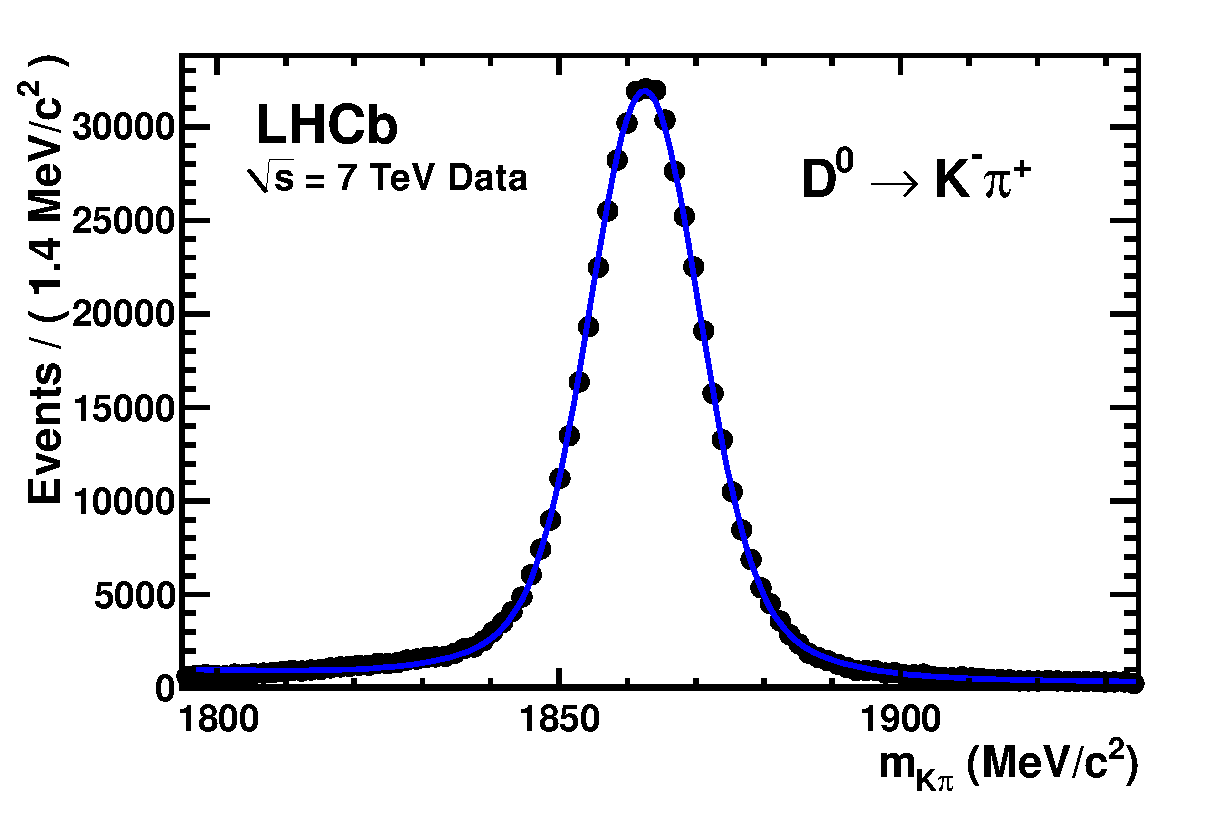
\includegraphics[width = 0.525\textwidth]{figs/detector/D0_Mass.eps}\put(-50,80){(a)}%
	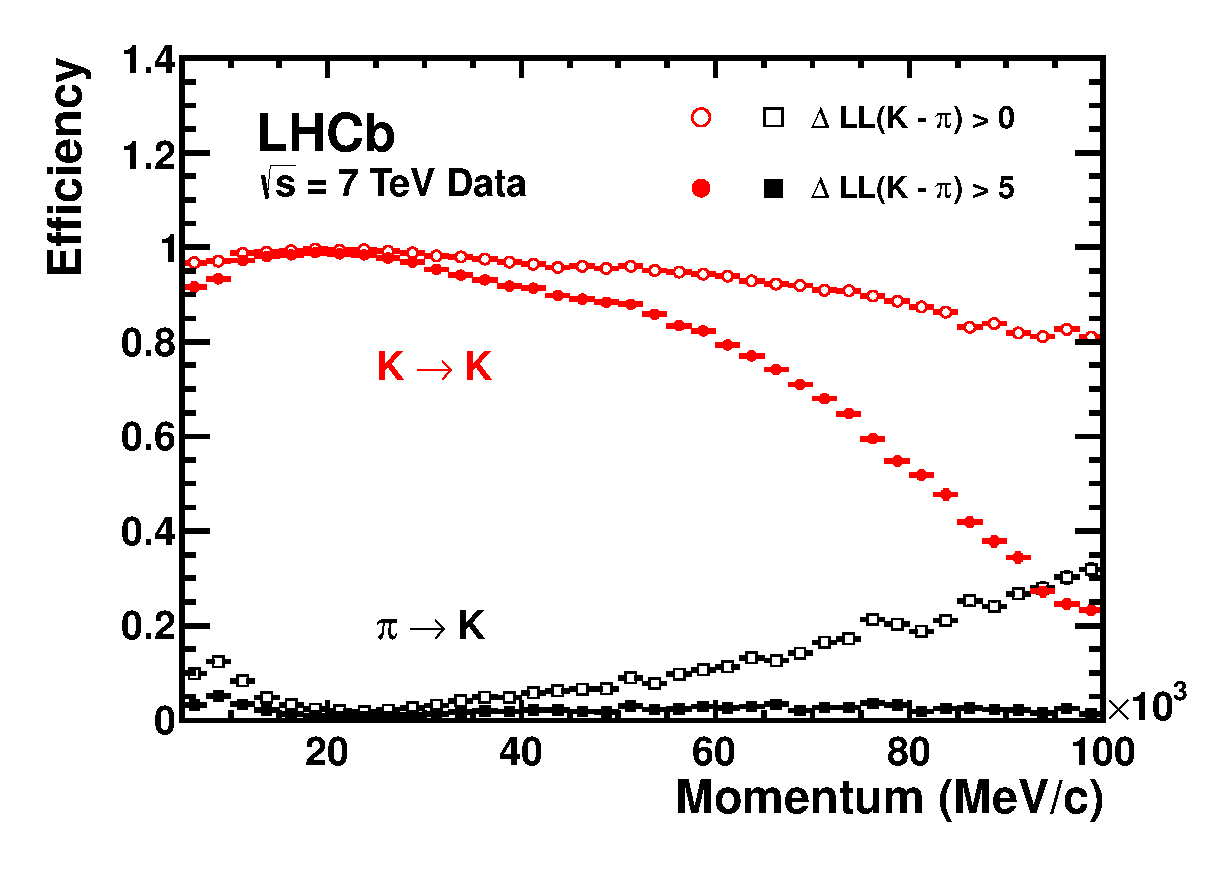
\includegraphics[width = 0.5\textwidth]{figs/detector/KandPi_2_K.eps}\put(-50,80){(b)}%
	\caption{ (a) Invariant mass distribution of $D^{0}$ data sample (in black) overlaid with fit to both background and signal (in blue). (b) An example of kaon ID (red) and misID (black) efficiency as a function of momentum under two \gls{PID} hypotheses, $\textrm{DLL{K}} > 0$ (empty)  and $\textrm{DLL{K}} > 5$ (filled). Both Figures from \cite{LHCb-DP-2012-003}.}
	\label{fig:richperf}
\end{figure}

%In search for $B^{0}$ and $B^{0}_{s}$ decaying to $h^{+}h^{-}$, where $h\in K, \pi$, $\pi^{+} \pi^{-}$ invariant mass spectra with and without \gls{PID} $\textrm{DLL{x}}$ requirements can be seen in~\autoref{fig:richnice}. These plots clearly demonstrate increase in sensitivity searching for $B^{0} \rightarrow \pi^{+} \pi^{-}$ signal amongst other components. 

%\begin{figure}[!h]
%	\centering
%	\includegraphics[width = 0.5\textwidth]{figs/detector/b2hhnopid.png}%
%	\includegraphics[width = 0.5\textwidth]{figs/detector/b2hhpid.png}%
%	\caption{ $\pi^{+} \pi^{-}$ invariant mass distributions obtained using kinematic constraints only (left) and also using \gls{PID} constraints (right) in order to isolate $B^{0} \rightarrow \pi^{+} \pi^{-}$ peak. This figure is taken from \cite{LHCb-PAPER-2012-002}. }  
%	\label{fig:richnice}
%\end{figure}


\section{Calorimetry }
\label{calosys}
As many other particle physics detectors, \Gls{LHCb} is equipped with series of subdetectors providing separation between electrons, pions and photons. This separation is achieved because different particles interact differently with the material, producing differently shaped showers. This part of the detector is not only integral to the way the \Gls{LHCb} trigger system works but it also provides a measurement of \DIFaddbegin \DIFadd{the }\DIFaddend energies of these objects.
All the subcomponents discussed here operate on the same principle. \DIFdelbegin \DIFdel{Passing particles }\DIFdelend \DIFaddbegin \DIFadd{Particles passing }\DIFaddend through the material emit light. The light from the scintillating material, which is created by absorbing the energy of the \DIFdelbegin \DIFdel{passing }\DIFdelend particle and re-emitted it in \DIFaddbegin \DIFadd{the }\DIFaddend form of light, is guided to photomultiplier tubes by wavelength shifting fibres.

Electrons, pions and photons firstly encounter two planes of scintillating tiles: the Scintillating Pad Detector (\Gls{SPD}), and the Preshower Detector (\Gls{PRS}) intersected by a wall of lead. The \Gls{SPD} senses the passage of charged particles as they emit light whereas neutral particles do not, making this subdetector \DIFaddbegin \DIFadd{able to }\DIFaddend distinguish between electrons and photons. The wall of lead initiates the electromagnetic shower, where photons are converted into electron-positron pairs, depositing sizable energy in the \Gls{PRS} allowing electron/pion separation. 

The Electromagnetic Calorimeter (\Gls{ECAL}) in \gls{LHCb} is based on a sampling shashlik-type technology, where scintillating tiles are alternated \DIFdelbegin \DIFdel{by }\DIFdelend \DIFaddbegin \DIFadd{with }\DIFaddend lead plates measuring the energy deposit of electromagnetic showers. As the best energy resolution requires full energy deposit of energetic photons along the \Gls{ECAL}, the thickness is equivalent to 25 radiation lengths. The resulting resolution of the \Gls{ECAL} is $\frac{\sigma_{E}}{E} = \frac{10\%}{\sqrt{E}} \oplus 1\%$, where $E$ is in \gev.

On the other hand, the Hadronic Calorimeter \Gls{HCAL} sandwiches iron instead of lead as the absorber with \DIFaddbegin \DIFadd{a }\DIFaddend thickness of 5.6 interaction length only, achieving a resolution of $\frac{\sigma_{E}}{E} = \frac{70\%}{\sqrt{E}} \oplus 10\%$ in beam tests. This poorer resolution however fulfils the requirements necessary for the main purpose of this detector, which is the hadron trigger. Away from the beampipe the granularity of cells is coarser to mirror the track occupancy as seen in~\autoref{fig:CaloGran}(a)(b). 

\begin{figure}[!h]
	\centering
	\includegraphics[width = 0.5\textwidth]{figs/detector/license/ECAL_crop.pdf}\put(-70,10){(a)}%%
	\includegraphics[width = 0.5\textwidth]{figs/detector/license/HCAL_crop.pdf}\put(-70,10){(b)}%%
	\caption{Granularity of (a) \Gls{ECAL} and (b) \Gls{HCAL} detectors. This is just a quarter view and that the black region is where the beam pipe is located. Figure from \cite{det_paper}. }  
	\label{fig:CaloGran}
\end{figure}




\section{Muon Stations }
\label{muonsys}
Muons are considered to be of fundamental importance to many flagship analyses by \Gls{LHCb}, such as the search for the rare $\B^{0}_{s} \rightarrow \mu^{+} \mu^{-}$ decay\cite{Aaij:2017vad}. Analysis of \Bmumumu of course relies heavily on \DIFaddbegin \DIFadd{a }\DIFaddend good performance of this part of \DIFaddbegin \DIFadd{the }\DIFaddend detector. Muon stations are positioned at the end of the detector, taking advantage of the fact that muons penetrate material better than any other particle type. 

\Gls{LHCb}'s five rectangular muon stations \Gls{muonstation} are positioned before and after \DIFaddbegin \DIFadd{the }\DIFaddend calorimetry system, with \DIFaddbegin \DIFadd{the }\DIFaddend first station M1 upstream of the \Gls{SPD}, and four stations (M2-M5) downstream of \Gls{HCAL} as shown in~\autoref{fig:MuonGran}. The M1 station consists of 12 sets of three gas electron 
multiplier foils (triple-GEMs) in the region closest to the beam pipe, resisting the highest dose of radiation due to the highest particle flux. Its main use lies in improving the measurement of $p_{T}$ in the hardware trigger. The M2-M5 stations each consist of 276 multi-wire proportional chambers (\Gls{MWPCs}) filled with an $\rm{Ar,CO_{2},CF_{4}}$ gas mixture. They are interlayered with 0.8\m iron walls, to provide a stopping target for all particles, other than muons with momentum higher than $6$ \gevc.

%In order to ease the accessibility, like in \Gls{VELO}, all the stations are split into two independent mechanical sides, also known A and C side.

Each half of a muon station is segmented into four increasingly larger regions away from the beam, R1 to R4.
 All the regions were constructed to cover the same acceptance, keeping the track occupancy constant across the station. The granularity of the readout is higher in the horizontal plane to take advantage of the magnet's horizontal bending plane.




\begin{figure}[!h]
	\centering
	\includegraphics[width = 1.0\textwidth]{figs/detector/sideview.pdf}%
	%\includegraphics[width = 0.5\textwidth]{figs/detector/b2hhpid.png}%
	\caption{(a) Layout of the muon detector x-z plane and (b) x-y plane. Figure from \cite{LHCb-DP-2012-002}. }  
	\label{fig:MuonGran}
\end{figure}

Both GEM and \Gls{MWPCs} operate on \DIFdelbegin \DIFdel{a }\DIFdelend \DIFaddbegin \DIFadd{the }\DIFaddend same principle. In each station, the position in the $x-y$ plane is determined by ionizing electrons that come from muons passing through the detector, which are then attracted either to the closest anode mesh or wire mesh. The trigger is fired if the corresponding rectangular region in each station registered a positive binary decision. This means \DIFdelbegin \DIFdel{an }\DIFdelend \DIFaddbegin \DIFadd{the }\DIFaddend efficiency of each station must be $\geq$99\% to give \DIFaddbegin \DIFadd{an }\DIFaddend overall 95\% trigger efficiency. %Geometrical layout covers $\approx$ 20\% muons originating in semileptonic $b$ decays.\mybox{\color{red}CERN-THESIS-2012-025.pdf from puig, i have to invedtigate}


\subsection{Muon Identification }
\label{muonID}
Apart from triggering events with high enough $p_{T}$ muons, the muon stations provide necessary \gls{PID} information for muon analyses. Offline variables mostly used for muon ID by analysts are
 \begin{itemize} 
	\DIFdelbegin %DIFDELCMD < \item{\textbf{IsMuon}: Boolean decision of muon candidates with momentum-dependent categorisation. Long tracks with $p>3$\gev/c are extrapolated to muon stations yielding $x-y$ coordinates in M2-M5, considering only tracks within acceptance. For each station, a search for hit information within an elliptical area defined by momentum, a field of interest (\Gls{FOI}), is performed. The hit requirements are summarized in~\autoref{tab:ismuontab}.}
%DIFDELCMD < 	\item{\textbf{muDLL}: Difference in log likelihoods computed using muon and non-muon hypothesis. These hypotheses are based on the proximity/distance $D^{2}$ of the track extrapolation into the muon stations and corresponding closest sensed hits in those stations. Muon-like particle will tend to have sharper distribution in $D^{2}$ as compared to other species. Protons were chosen to be the other species for the calibration purposes. They give a broader distribution as they originate either as punch-through protons (protons coming from showers not fully contained in the \gls{HCAL}), protons having coincident hit position to a true muon, or random hits.}
%DIFDELCMD < 	%%%
\DIFdelend \DIFaddbegin \item{\textbf{IsMuon}: Boolean decision of muon candidates with momentum-dependent categorisation. Long tracks with $p>3$\gev/c are extrapolated to muon stations yielding $x-y$ coordinates in M2-M5, considering only tracks within the acceptance. For each station, a search for hit information within an elliptical area defined by momentum, a field of interest (\Gls{FOI}), is performed. The hit requirements are summarized in~\autoref{tab:ismuontab}.}
	\item{\textbf{muDLL}: Difference in log likelihoods computed using a muon and non-muon hypothesis. These hypotheses are based on the prox imity/distance, $D^{2}$, of the track extrapolation into the muon stations and corresponding closest sensed hits in those stations. Muon-like particles will tend to have a sharper distribution in $D^{2}$ as compared to other species. Protons were chosen to be the other species for the calibration purposes. They give a broader distribution as they originate either as punch-through protons (protons coming from showers not fully contained in the \gls{HCAL}), protons having the same hit position as true muon, or random hits.}
	\DIFaddend \item{\textbf{DLLmu}}:  For each track \DIFdelbegin \DIFdel{a }\DIFdelend \DIFaddbegin \DIFadd{the same }\DIFaddend global likelihood is produced, by \DIFdelbegin \DIFdel{combination of }\DIFdelend \DIFaddbegin \DIFadd{combining the }\DIFaddend muon and non-muon \DIFdelbegin \DIFdel{likelihood }\DIFdelend \DIFaddbegin \DIFadd{likelihoods }\DIFaddend from \textbf{muDLL}, with the \Gls{RICH} different mass hypothesis likelihoods, and \DIFaddbegin \DIFadd{the }\DIFaddend calorimetry likelihood exploiting \DIFaddbegin \DIFadd{information about }\DIFaddend the energy deposits\DIFdelbegin \DIFdel{information}\DIFdelend . Like in the \Gls{RICH} likelihoods, the default hypothesis corresponds to separation between the muon and pion hypotheses.    

 \end{itemize} 

\noindent \DIFdelbegin \DIFdel{Other variables which are extensively }\DIFdelend \DIFaddbegin \DIFadd{In the }\Bmumumu \DIFadd{analysis }\texttt{\DIFadd{IsMuon}} \DIFadd{and }\texttt{\DIFadd{DLLmu}} \DIFadd{variables are used to identify muons. On the top, other variables, which are }\DIFaddend used for muon \DIFdelbegin \DIFdel{particle identification in }\DIFdelend \DIFaddbegin \DIFadd{identification in the }\DIFaddend search for \Bmumumu\DIFaddbegin \DIFadd{, }\DIFaddend are described in~\autoref{otherpid}. \DIFaddbegin \DIFadd{The use of several variables for muon identification is done as they are mostly complimentary, exploiting different information from different parts of the detector. 
}\DIFaddend 

\begin{table}[!h]
	\centering
	\hspace*{-0.8cm}
	\begin{tabular}{c c}
		\toprule
		Particle Momentum $p$  & Hits in Muon Stations \\ \hline
		3 \gev/c <$p$<6 \gev/c & M1 $\&$ M2\\
		6 \gev/c <$p$<10 \gev/c & M1 $\&$ M2 $\&$ (M3 $||$ M4) \\
		10 \gev/c <$p$ & M1, M2, M3 and M4 \\ \bottomrule      
	\end{tabular}
	\caption{Momentum-dependent definition \texttt{IsMuon} variable.}
	\label{tab:ismuontab}
\end{table}   

\subsection{Muon Identification Performance}
\label{muonperf}
As for hadron performance measurements, the muon ID performance is determined using the high statistics decay channel $J/\psi \rightarrow \mu^{+} \mu^{-}$ with a \textit{tag and probe} method. MisID rates \DIFdelbegin \DIFdel{of }\DIFdelend \DIFaddbegin \DIFadd{for }\DIFaddend kaons and pions are computed using the same decay channels, which were used for \DIFaddbegin \DIFadd{the }\DIFaddend identification of hadrons, $D^{*+} \to D^{0}(\kaon^{-}\pip)\pip$. The summary of \texttt{IsMuon} ID and misID rates are presented in~\autoref{fig:MuonID}. \DIFdelbegin \DIFdel{Very }\DIFdelend \DIFaddbegin \DIFadd{A very }\DIFaddend high ID rate (above 90\%) for relatively low misID probability (below 10\%) is key to analyses with muons in \DIFdelbegin \DIFdel{a }\DIFdelend \DIFaddbegin \DIFadd{the }\DIFaddend final state. \DIFdelbegin \DIFdel{But the least performing are the }\DIFdelend \DIFaddbegin \DIFadd{The identification rate for the }\DIFaddend low $p_{T}$ muons \DIFdelbegin \DIFdel{where the identification }\DIFdelend suffers because these muons can end up outside of the \gls{LHCb} acceptance\DIFdelbegin \DIFdel{and misID }\DIFdelend \DIFaddbegin \DIFadd{. MisID }\DIFaddend rates for kaon and pions are significantly higher in \DIFaddbegin \DIFadd{the }\DIFaddend low momenta region as the dominant process \DIFdelbegin \DIFdel{causing this are }\DIFdelend \DIFaddbegin \DIFadd{for this occurence is }\DIFaddend muons from decay-in-flight.   

\begin{figure}[!h]
	\includegraphics[width = 0.5\textwidth]{figs/detector/dllFit_mu_IMvsPvsPt.pdf}%
	\includegraphics[width = 0.5\textwidth]{figs/detector/dllFit_P_IMvsPvsPt.pdf}%
       \newline
	\includegraphics[width = 0.5\textwidth]{figs/detector/dllFit_pi_IMvsPvsPt.pdf}%
	\includegraphics[width = 0.5\textwidth]{figs/detector/dllFit_ka_IMvsPvsPt.pdf}%
	\caption{(a) Probability of correctly identifying muons as a function of momentum \DIFdelbeginFL \DIFdelFL{$p$ }\DIFdelendFL in \DIFdelbeginFL \DIFdelFL{the }\DIFdelendFL bins of $p_{T}$ for $J/\psi \rightarrow \mu^{+} \mu^{-}$ with \DIFaddbeginFL \DIFaddFL{an }\DIFaddendFL \texttt{IsMuon} constraint. (c) Probability of incorrectly identifying \DIFaddbeginFL \DIFaddFL{a }\DIFaddendFL pion (b) proton and (d) kaon as \DIFaddbeginFL \DIFaddFL{a }\DIFaddendFL muon with \texttt{IsMuon}. This figure is taken from \cite{LHCb-DP-2013-001}. }  
	\label{fig:MuonID}
\end{figure}


\section{Trigger }
\label{triggerchap}
Big-data physics experiments have to make decisions on what kind of data they want to keep. The choice of interesting events is performed by a series of decisions, which is known as the trigger. The \Gls{LHCb} trigger system was build around constraints posed by the run conditions, read-out capabilities and available disk space. In Run \Rn{1} and Run \Rn{2} \gls{LHCb} has at its disposal the multistage trigger consisting of a hardware-based level 0 trigger (\Gls{L0}) and a software-based high level trigger (\Gls{HLT}).

In the end, selected events have their trigger decisions categorized. An event where the signal candidate caused the trigger to fire is known \DIFdelbegin \DIFdel{to be }\DIFdelend \DIFaddbegin \DIFadd{as }\DIFaddend Trigger on Signal (\Gls{TOS}). An event where it is a non-signal like particle causing the trigger decision to occur \DIFdelbegin \DIFdel{, }\DIFdelend \DIFaddbegin \DIFadd{is labelled as }\DIFaddend Trigger Independent of Signal (\Gls{TIS})\DIFdelbegin \DIFdel{is labelled}\DIFdelend . Finally, if only \DIFdelbegin \DIFdel{by }\DIFdelend a combination of signal particle(s) together with other \DIFdelbegin \DIFdel{particle's properties }\DIFdelend \DIFaddbegin \DIFadd{particles }\DIFaddend in the event \DIFdelbegin \DIFdel{produce }\DIFdelend \DIFaddbegin \DIFadd{produces }\DIFaddend an affirmative decision, then these events are categorized as \Gls{TIS} $\&$ \Gls{TOS} = \Gls{TISTOS}.

\Gls{L0} reduces the rate of data from 40 \mhz to 1 \mhz by employing five trigger decisions, also known as lines. The first three lines make \DIFaddbegin \DIFadd{a }\DIFaddend decision using calorimeter information about the transverse energy, $E_{T}$, \DIFaddbegin \DIFadd{and }\DIFaddend whether it is \DIFaddbegin \DIFadd{a }\DIFaddend photon, electron or hadron causing the shower energy deposit. Two other lines \DIFdelbegin \DIFdel{are reading }\DIFdelend \DIFaddbegin \DIFadd{read }\DIFaddend out information from the muon system by looking for  \DIFdelbegin \DIFdel{transverse momentum, }\DIFdelend $p_{T}$, of muon and dimuon (two muon tracks) objects. \DIFdelbegin \DIFdel{Efficiencies }\DIFdelend \DIFaddbegin \DIFadd{The efficiencies }\DIFaddend of the L0 muon triggers are evaluated using $B^{+} \rightarrow (J/\psi \rightarrow \mu^{+} \mu^{-}) K^{+}$ decays and can be seen in~\autoref{fig:L0Perf}(a). The hadron trigger efficiency in different decay channels can be seen in~\autoref{fig:L0Perf}(b). 


\begin{figure}[!h]
	\centering
	\includegraphics[width = 0.5\textwidth]{figs/detector/Fig1_L0MuonEff_PT.pdf}\put(-50,90){(a)}%
	\includegraphics[width = 0.5\textwidth]{figs/detector/Fig21_L0Hadron_PT.pdf}\put(-50,90){(b)}%
	%\includegraphics[width = 0.5\textwidth]{figs/detector/b2hhpid.png}%
	\caption{ (a) \Gls{TOS} efficiency as a function of $p_{T}$ for muon-based decisions. (b) \Gls{TOS} efficiency for different decays using L0 hadron trigger lines. Figures from \cite{Albrecht:2013fba}. }  
	\label{fig:L0Perf}
\end{figure}


 The software-based \Gls{HLT} then further reduces the rate from 1 \mhz down to $5$ \khz which can be recorded to long-term storage. The first stage of the \Gls{HLT}, (\Gls{HLT1}), performs limited track reconstruction and hence makes a decision based on the presence of charged particles in the event. \Gls{HLT1} uses \Gls{VELO} hits to reconstruct \Gls{PV}s and \Gls{VELO} tracks by using 3D pattern recognition. As \Gls{LHCb}'s primary mission is to study decays of hadrons containing $b$ and $c$ quark, \Gls{HLT1} will make \DIFaddbegin \DIFadd{a }\DIFaddend decision based on the track being displaced (having \DIFaddbegin \DIFadd{a }\DIFaddend high \Gls{IP}) with respect to the \Gls{PV}. For events selected by the \texttt{L0Muon}, an attempt is made to match the \Gls{VELO} tracks to hits observed in the vertical plane in the muon chambers, where the magnetic field of the dipole will not make them bend. By computing the track $\chi^2$, the potential muon track candidates are selected. Finally, the \Gls{VELO} tracks and muon tracks are extrapolated into the \Gls{OT} or \Gls{IT} trackers, allowing for so called \textit{forward tracking}, whereby $p$ and $p_{T}$ requirements are imposed to reduce processing time. Each track is then fitted with  a fast Kalman filter providing the $\chi^2$ of the fit. The corresponding performance of \DIFaddbegin \DIFadd{the }\DIFaddend \Gls{HLT1} trigger lines are shown in~\autoref{fig:Hlt1Perf}(a)(b).


\begin{figure}[!h]
	\centering
	\includegraphics[width = 0.5\textwidth]{figs/detector/Fig3_Hlt1MuonEff_PT.pdf}\put(-50,140){(a)}%
	\includegraphics[width = 0.5\textwidth]{figs/detector/Fig5_Hlt1TrackAllL0_PT.pdf}\put(-50,140){(b)}%
	%\includegraphics[width = 0.5\textwidth]{figs/detector/b2hhpid.png}%
	\caption{ \Gls{HLT1} efficiencies of the corresponding triggers using the same proxy as in~\autoref{fig:L0Perf}. Figures from \cite{Albrecht:2013fba}. }  
	\label{fig:Hlt1Perf}
\end{figure}

The second stage \Gls{HLT2} reduces the rate to 5 \khz that can be safely written to disk. \Gls{HLT2} consists of a series of decisions based on a full reconstruction of either groups of decays or specific decay modes. \textit{Topological triggers} exploit the vertex and track information (topology) of $b$-hadron decays. By employing multivariate techniques 2-,3- or 4-body decays that are well separated from the \Gls{PV} are reconstructed. To account for decays where a final state particle is not fully reconstructed, the corrected mass (will be defined in~\autoref{eq:corrm}) serves as an input variable in the the \Gls{BDT}. Dedicated lines are also written to reconstruct muon and dimuon channels allowing for both prompt $J/\psi$ and $B\rightarrow J/\psi X$ studies. Finally there are \textit{Exclusive triggers} concentrating on selecting events with $D$ mesons. They perform \DIFaddbegin \DIFadd{a }\DIFaddend selection which is very similar to the offline selection but without \Gls{PID} cuts.% and with \textit{prescales} required, where only a certain fraction of events is allowed to pass through.



Between the Run \Rn{1} and Run \Rn{2} period there has been a change in how the software trigger operates, which can be seen in~\autoref{fig:TriggerChange}. As more computing resources were introduced for both \Gls{HLT1} and \Gls{HLT2}, \Gls{LHCb} took advantage in upgrading the trigger system by introducing an update of \DIFaddbegin \DIFadd{the }\DIFaddend calibration and alignment constants of the relevant subdetectors before the data is sent to permanent disk. \textit{Online reconstruction}, defined as being produced at the trigger farm, became the same as the \textit{offline reconstruction}, defined as reconstruction made when data reached the permanent disk. Hence, there is \DIFdelbegin \DIFdel{enhancement of }\DIFdelend \DIFaddbegin \DIFadd{an enhancement of the }\DIFaddend available information, such as the \Gls{PID} in the \Gls{HLT}, which can then be used at the trigger level. 


\begin{figure}[!h]
	\centering
	\includegraphics[width = 0.5\textwidth]{figs/detector/LHCb_Trigger_RunIAlg.pdf}%
	\includegraphics[width = 0.5\textwidth]{figs/detector/LHCb_Trigger_RunII.pdf}%
	%\includegraphics[width = 0.5\textwidth]{figs/detector/b2hhpid.png}%
	\caption{Trigger scheme differences between Run \Rn{1} and Run \Rn{2}. Figures from \cite{triggerscheme}.}  
	\label{fig:TriggerChange}
\end{figure}


\section{Simulation }
\label{simulationchap}
In order to optimise the event selections, determine efficiencies and model the backgrounds, a full Monte Carlo Simulation \Gls{MC} can be produced starting from simulation of the $pp$ collision to detector readout of the decay of interest produced. 
The $pp$ collisions within the \Gls{LHCb} configuration \cite{Belyaev:2011zza} are simulated with Pythia 6.4 \cite{pythia6} and Pythia 8.1 \cite{pythia8}. \Gls{LHCb} specific settings are mostly related to running conditions: luminosity, number of collisions per bunch crossing as well as contamination from other bunches, \textit{spill-over}. 

In the $pp$ collision, the $b$ and $c$ production mechanisms are simulated and then the following $b\bar{b}$ or $c\bar{c}$ pair is hadronized into hadrons of interest. In this thesis and the analysis presented, the \Bp meson is the hadron of interest. Hadrons are then further decayed using EVTGEN \cite{Lange:2001uf} into the chosen decay products. At this stage, different physics models or inputs from theory can be configured. % At the same time some initial CPU-friendly selection is established, usually requiring the hadrons to be contained within the forward detector's acceptance.
In order to account for the effects of \Gls{QED} radiative corrections, the PHOTOS \cite{photos} algorithm can be used. All of this combined establishes \textit{the generator-level simulation} of LHCb.


In the next phase, \textit{detector simulation}, the interactions of \DIFdelbegin \DIFdel{the }\DIFdelend all the particles with the detector, transport, as well as detector's response are simulated using the C++ GEANT4 toolkit \cite{Geant4},\cite{Agostinelli:2002hh}. \Gls{LHCb}'s interface to GEANT4 is detailed in Ref\cite{Clemencic:2011zza}. 

\subsection{Differences in Simulation and Data}
\label{detpid}
Despite the complexity and best intention of the \Gls{LHCb} simulation, there are several shortcomings that require corrections.
The most affected variables necessary for physics analyses that one needs to consider are \Gls{IP} resolution, track reconstruction efficiencies, \Gls{PID} variables and track occupancy.

The \Gls{IP} resolution shows a better trend in the simulation then in the data due to the mismodelling of the material description \DIFdelbegin \DIFdel{of }\DIFdelend \DIFaddbegin \DIFadd{in }\DIFaddend the \Gls{VELO} simulation. As shown in~\autoref{fig:IPRES}(a)(b)  the \Gls{IP} resolution does greatly differ depending \DIFaddbegin \DIFadd{on }\DIFaddend the variation of material density of \Gls{VELO}. Around $\phi=\pm\pi/2$, where the two \Gls{VELO} parts overlap, the material difference causes the discrepancy. It can be corrected either by reweighting to data or by smearing the resolution with a Gaussian distribution.

\begin{figure}[!h]
	\centering
	\includegraphics[width = 0.5\textwidth]{figs/detector/IPXRes-Vs-InversePT-Compare2012DataToMC.pdf}\put(-50,60){(a)}%
	\includegraphics[width = 0.5\textwidth]{figs/detector/IPXRes-Vs-Phi-Compare2011DataToMC.pdf}\put(-50,60){(b)}%
	\caption{ (a) \Gls{IP} resolution in \DIFaddbeginFL \DIFaddFL{the }\DIFaddendFL x-direction comparing the data and simulation \DIFdelbeginFL \DIFdelFL{output }\DIFdelendFL for \DIFaddbeginFL \DIFaddFL{the }\DIFaddendFL 2012 data-taking period. (b) \Gls{IP} resolution in \DIFaddbeginFL \DIFaddFL{the }\DIFaddendFL x-direction comparing the data and simulation \DIFdelbeginFL \DIFdelFL{output }\DIFdelendFL for \DIFaddbeginFL \DIFaddFL{the }\DIFaddendFL 2011 data-taking period as a function of angle, $\phi$. Figures from \cite{LHCbVELOGroup:2014uea}. }  
	\label{fig:IPRES}
\end{figure}


Track reconstruction efficiency is also not reproduced very well in certain \DIFdelbegin \DIFdel{kinematical }\DIFdelend \DIFaddbegin \DIFadd{kinematic }\DIFaddend bins, again due to modelling of scattering interactions.

The most critical problem that needs to be addressed in the presented analysis \DIFdelbegin \DIFdel{are }\DIFdelend \DIFaddbegin \DIFadd{is }\DIFaddend the inaccuracies of the \Gls{PID} variables, which are mismodelled in the simulation. \DIFdelbegin \DIFdel{The origin of this }\DIFdelend \DIFaddbegin \DIFadd{This }\DIFaddend problem arises as a consequence of \DIFaddbegin \DIFadd{the }\DIFaddend much lower estimate of low momentum tracks in the detector\DIFaddbegin \DIFadd{, }\DIFaddend making the photoelectron background underestimated. This results in better \DIFdelbegin \DIFdel{performance of separation power }\DIFdelend \DIFaddbegin \DIFadd{separation }\DIFaddend in simulation and is corrected using \DIFaddbegin \DIFadd{a }\DIFaddend data calibration. 

Therefore the \gls{PID} efficiency is usually obtained from \DIFaddbegin \DIFadd{the }\DIFaddend data. More specifically, this is done by using high-yield and relatively background-free calibration channels, where the species of the particle can be deduced from kinematics of the decay. \DIFdelbegin \DIFdel{Standard }\DIFdelend \DIFaddbegin \DIFadd{A standard }\DIFaddend set of these channels are "housed" in a \texttt{PIDCalib} package \cite{Anderlini:2202412}. \DIFdelbegin \DIFdel{In }\DIFdelend \DIFaddbegin \DIFadd{With }\DIFaddend this package, \DIFaddbegin \DIFadd{the }\DIFaddend \gls{PID} efficiency can be computed in a given kinematic region of interest. 


